% !TeX root = ../thuthesis-example.tex

\chapter{实际场景中的应用}

本节主要介绍随机标准化层在两个实际场景——医疗影像诊断和风速预测中的应用情况,以及算法库集成的相关工作。

\section{医疗影像诊断}

\subsection{应用背景}

2020年至今,新冠肺炎在世界范围内流行开来,对全人类的生命健康安全带来了巨大的威胁。在这场疫情中,各行各业都为抗击疫情做出了贡献,而计算机视觉技术则在新冠肺炎的辅助诊断领域有着
不错的效果。对于很多疾病,首先需要通过X光透射、CT扫描或者核磁共振等手段对有疑似病灶的部位进行检查,有经验的医生能通过检查得到的图像进行快速诊断。但是当疫情快速蔓延时,相关专业人士
的数量往往不足以支撑大量的疾病诊断,这时便可以借助计算机视觉技术进行辅助诊断。

\begin{figure}
  \centering
  \subcaptionbox{Infiltration, Nodule and Mass}
    {\includegraphics[width=0.3\linewidth]{figures/nih/1.png}}
  \subcaptionbox{Effusion, Infiltration, Nodule and Consolidation}
    {\includegraphics[width=0.3\linewidth]{figures/nih/2.png}}
  \subcaptionbox{Effusion, Infiltration, Atelectasis and Edema}
    {\includegraphics[width=0.3\linewidth]{figures/nih/3.png}}
  \caption{NIH Chest X-ray数据集示例}
  \label{fig:nih}
\end{figure}

医疗影像数据相比传统的图像数据来说,最大的特点便是数据的采集非常耗时耗力,同时数据的标注也非常困难,导致有标注的数据更加稀缺,如何利用稀少但是珍贵的有标注数据来提高模型的诊断准确率,是
计算机视觉技术在医疗影像数据领域的一大难题。除此之外,医疗影像数据还有采集方式与常见的RGB图像有一定区别、病患相关的数据需要脱敏处理、不同疾病的拍摄部位区别很大等诸多问题。因此医疗影像诊断这一
任务,是检验计算机视觉相关算法落地能力的一个重要场景。

\subsection{实验设计}

本节选用了两个基于肺部X光和CT影像的医疗数据集——NIH Chest X-ray~\citep{wang2017chestxray}和COVID-CT~\citep{he2020sample}进行实验。NIH Chest X-ray包含了来自约$3$万名患者
超过$11$万张的肺部正面X光影像,共有$14$种肺部疾病类别(每一张图像可能属于多个类别),是一个多标签的图像分类任务;COVID-CT则包含了来自$216$名新冠肺炎患者的$349$张CT影像,以及大量
正常人的CT影响作为对照,是一个图像二分类任务。图~\ref{fig:nih}和图~\ref{fig:covid}分别展示了两个数据集内的一些图片示例。可以看出,医疗影像相比传统的图像数据来说细节更多,更难以区分,
进行诊断需要极强的专业知识,因此也给了深度学习相关技术开阔的发挥空间。


\begin{figure}
  \centering
  \subcaptionbox{阴性}{
    \includegraphics[width=0.45\linewidth]{figures/covid-ct/1.png}
    \includegraphics[width=0.45\linewidth]{figures/covid-ct/2.png}
  }
  \subcaptionbox{阳性}{
    \includegraphics[width=0.45\linewidth]{figures/covid-ct/3.png}
    \includegraphics[width=0.45\linewidth]{figures/covid-ct/4.png}
  }
  \caption{COVID-CT数据集示例}
  \label{fig:covid}
\end{figure}


NIH Chest X-ray数据集的数据来自于很多个国家和地区,因此包含着上万条数据用于训练,但是在实际场景中医疗数据的采集耗时耗力,还要考虑信息脱敏等额外隐患,所以很难拥有如此多的数据。所以在本文的实验中,
我们对NIH Chest X-ray数据集进行了三个比例的数据采样——$5\%$、$10\%$和$15\%$,以验证在更符合实际场景的情况下,StochNorm以及一系列主流的模型微调方法能否取得更好的效果。由于数据可能包含多个标签,
作为一个多标签的分类任务,本文使用在14种疾病的的平均AUC作为验证指标,预训练模型选择ResNet-50。

相比起NIH Chest X-ray数据集而言,COVID-CT数据集则更贴近现实场景下的医疗数据集、由于新冠肺炎是近年来新出现的疾病,所以数据集中只包含了几百张新冠肺炎的正样本CT影像,能够更好地验证模型微调方法在实际场景中
是否有作用,是否能够更大程度地利用预训练模型的知识,在稀少却很珍贵的数据上训练得到更好的效果。本文依然比较了StochNorm以及一系列主流的模型微调方法,验证指标选择AUC,预训练模型选择ResNet-50。

\subsection{实验结果} 

两个数据集上的实验结果如表~\ref{table:chexray}和表~\ref{table:covid-ct}所示。Raghu\citep{raghu2019transfusion}等人的工作发现,由于广泛使用的预训练模型使用的数据和实际场景中的医疗数据之间有着巨大的领域差异,
因而在这些医疗数据集上,传统的$L_2$模型微调无法取得足够明显的提升。本文的实验也证实了,很多在常规数据集上表现较好的基于正则化约束项的模型微调方法,在医疗数据集上反而会带来负收益。但是相反的,作为一种结构化的隐式正则方法,
通过简单地将BatchNorm替换为StochNorm,能够在COVID-CT数据集上有$\textbf{3.13\%}$的AUC提升,在NIH Chest X-ray数据集的三个采样比例下也取得了平均$\textbf{1.1\%}$的AUC提升。这说明了,在数据量不够充足的情况下,模型微调的方法依然有很多提升的空间。

\begin{table*}[h]
	\begin{center}
  \caption{NIH Chest X-ray数据集实验结果}
	\label{table:chexray}
    \begin{tabular}{lccc}
        \toprule
        \multirow{2}*{方法} & \multicolumn{3}{c}{数据采样比例} \\
        \cmidrule(r){2-4}
          & $5\%$ & $10\%$ & $15\%$ \\
        \midrule
        Baseline($L_2$) & $70.37\pm0.31$ & $75.85\pm0.22$ & $76.64\pm0.11$ \\
        $L_2$-SP \citep{xuhong2018explicit} & $70.02\pm0.27$ & $72.73\pm0.41$ & $75.71\pm0.22$  \\
        DELTA \citep{li2018delta} & $70.99\pm0.19$ & $74.35\pm0.20$ & $75.97\pm0.17$ \\
        BSS \citep{chen2019catastrophic} & $69.86\pm0.12$ & $73.27\pm0.19$ & $76.10\pm0.23$  \\
        \cmidrule(r){1-4}
        \textbf{StochNorm} & $\textbf{72.50}\pm\textbf{0.26}$ & $\textbf{76.48}\pm\textbf{0.15}$ & $\textbf{77.01}\pm\textbf{0.21}$ \\
        \bottomrule
    \end{tabular}
	\end{center}
\end{table*}


\begin{table*}[h]
	\begin{center}
  \caption{COVID-CT数据集实验结果}
	\label{table:covid-ct}
    \begin{tabular}{lccccccccc}
        \toprule
        Baseline($L_2$) & $L_2$-SP \citep{xuhong2018explicit} & DELTA \citep{li2018delta} & BSS \citep{chen2019catastrophic} &  \textbf{StochNorm}\\
        \midrule
        $87.30\pm0.20$ & $85.11\pm0.13$ & $87.79\pm0.24$ & $88.52\pm0.31$ & $90.43\pm0.15$\\
        \bottomrule
    \end{tabular}
	\end{center}
\end{table*}

\section{金风风速预测}

\subsection{应用背景}

2020年9月我国明确提出“双碳”战略,即2030年“碳达峰”与2060年“碳中和”目标。对于燃烧煤炭进行火力发电这种传统的发电方式,碳排放量极大,与“双碳”战略相斥,需要被逐步取代,而诸如利用风能等
清洁能源进行发电的方式逐渐受到重视。我们国家地大物博,风能资源丰富,在许多地方都有面积巨大的风场,如何利用这些风场高效发电,是当下的热点问题。对于传统火力发电而言,发电功率取决于
煤炭燃烧的速率,能够被人为地控制,而风力发电的功率则主要取决于风速,具有很强的随机性和不可控性。因此,如果能较为准确地预测未来的风速变化趋势,对于电厂进行统筹规划来说又很大的意义。

\begin{figure}
  \centering
  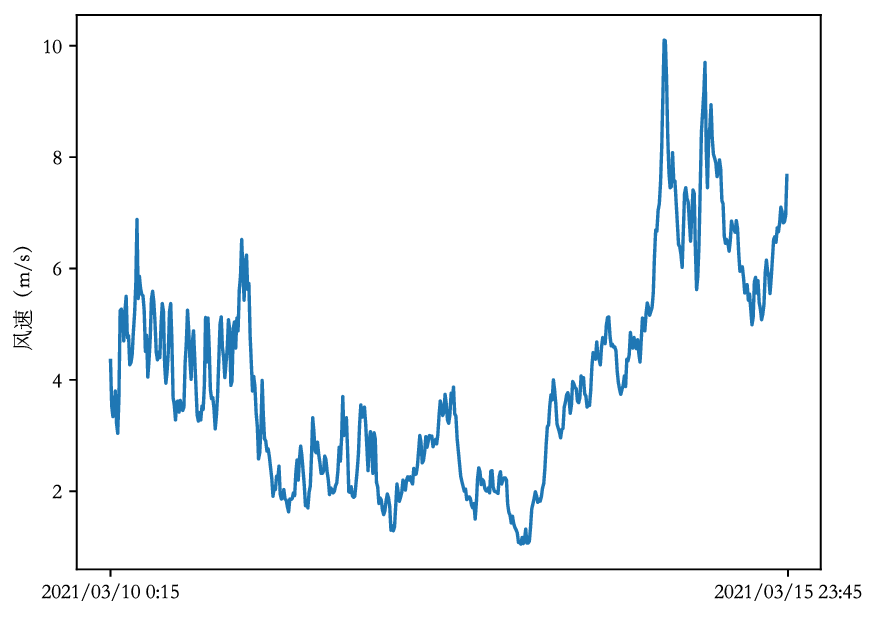
\includegraphics[width=0.75\linewidth]{figures/wind.pdf}
  \caption{金风风速数据示例}
  \label{fig:goldwind}
\end{figure}

在不同地区、不同季节、不同时间风场的风速都有所不同,而风场的各种气象特征都与风速的变化息息相关。当下的前沿工作主要采用数值天气预报来预测风速,数值天气预报可以通过卫星、雷达、气象站等方式获取,
包括不同高度的温度、湿度、压强、云量等气象指标,为接下来进行风速预测提供了数据基础。风速预测一般按照预测时长分为三类:短期、中期和长期风速预测,预测的时间区间从几天到几个月甚至一年以上,相应的
预测精度要求也会随时间增加而降低。

本文涉及的项目为金风风速预测项目,主要的目标为进行短期的风速预测,即预测$3km\times3km$空间内在未来$8$天左右的风速情况,时间间隔为$15$分钟,属于精度要求较高的一种风速预测任务。图~\ref{fig:goldwind}
为2021年3月的风速观测曲线。对于该任务而言,主要面临的困难在于金风风场的风速数据变化大、抖动多、噪声多等问题,气象预报数据种类非常多,并且存在不可避免的误差,很容易在训练数据上出现过拟合的现象,缺乏泛化性和
迁移性。同时,由于数据中同时包含气象预报数据和风速数据,与学术界时间序列研究的问题设定有很多不同,需要针对实际场景进行设计与调整,为深度学习算法的实际落地带来了很多阻碍。

\begin{figure}
  \centering
  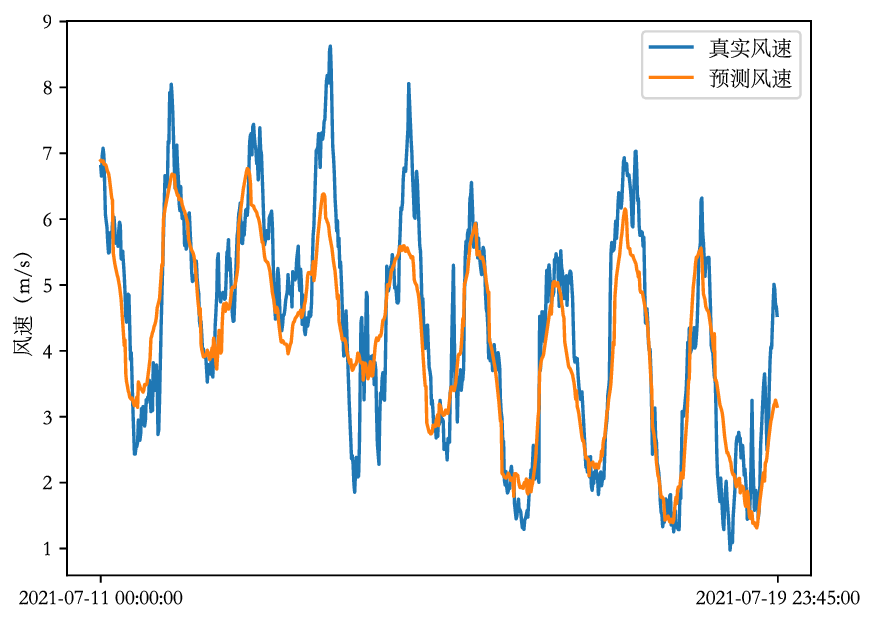
\includegraphics[width=0.75\linewidth]{figures/wind2.pdf}
  \caption{金风风速真实曲线与预测曲线}
  \label{fig:pred}
\end{figure}

\begin{table*}[h]
	\begin{center}
  \caption{金风风速预测数据集实验结果}
	\label{table:goldwind}
    \begin{tabular}{ccccc}
        \toprule
        训练数据 & 测试数据 & 金风基线指标 & Baseline &  Baseline+\textbf{StochNorm}\\
        \midrule
        03/01-05/30 & 05/31-06/10 & 1.433 & 1.337 & 1.264 \\
        03/11-06/10 & 06/11-06/20 & 1.183 & 0.777 & 0.789 \\
        03/21-06/20 & 06/21-06/30 & 1.090 & 1.225 & 1.181 \\
        \cmidrule(r){1-5}
        04/01-06/30 & 07/01-07/10 & 1.093 & 0.946 & 1.066 \\
        04/11-07/10 & 07/11-07/20 & 1.159 & 0.830 & 0.794 \\
        04/21-07/20 & 07/21-07/30 & 1.184 & 1.511 & 1.474 \\
        \cmidrule(r){1-5}
        05/01-07/30 & 07/31-08/10 & 1.302 & 1.393 & 1.271 \\
        05/11-08/10 & 08/11-08/20 & 1.014 & 1.055 & 0.908 \\
        05/21-08/20 & 08/21-08/30 & 1.084 & 1.030 & 0.874 \\
        \cmidrule(r){1-5}
        06/01-08/30 & 08/31-09/10 & 1.038 & 0.880 & 0.859 \\
        06/11-09/10 & 09/11-09/20 & 1.262 & 1.200 & 1.339 \\
        06/21-09/20 & 09/21-09/30 & 1.201 & 1.081 & 1.071 \\
        \midrule
        \multicolumn{2}{c}{平均值} & 1.170 & 1.105 & 1.074 \\
        \bottomrule
    \end{tabular}
	\end{center}
\end{table*}

\subsection{实验设计}

本节选择了金风风速预测数据集中的广西风场数据作为实验数据集。数据集包含了2021年3月至9月共计7个月内的气象数据预报数据,比如压强、温度、湿度等气象数据,以及每个时间点测量点测
量得到的风速。本文选择连续3个月的气象数据以及风速作为深度神经网络的训练输入,之后以接下来10天的气象预报数据作为测试输入,来预测接下来10天每个时间节点的实时风速,属于包含
时序数据的回归问题。训练数据在3到9月的时间节点上,以三个月为训练区间,10天为间隔做平移,共得到12组训练-测试数据对。深度神经网络结构方面使用三层MLP作为回归器,通过某一时刻的气象预报
数据来回归预测相应的风速,同时加入Transformer利用预测的历史风速和真实的历史风速数据,捕捉风速之间的时序关系,从而基于未来的气象预报数据预测风速。为了验证StochNorm在该场景下的效果,
本文将原网络结构中的标准化层替换为StochNorm,验证指标为10天内风速预测的均方根误差(Root Mean Squared Error, RMSE)。

\subsection{实验结果}

实验结果如表~\ref{table:goldwind}所示,可以看出MLP+Transformer的网络结构相比金风提供的基线指标有一定的提升,而在更换为StochNorm之后,模型的RMSE有了进一步的下降,12组数据上相比基线
指标的相对提升平均为$\textbf{8.21\%}$。通过进一步的分析发现,由于风速与同一时刻的很多气象特征有着强相关性,使得在某一时间训练的模型很容易出现过拟合的现象,而由于不同时刻的风速随机性较强,
过拟合的模型在训练时间段以外的效果可能会变差。图~\ref{fig:pred}展示了预测的风速曲线与实际风速曲线的比较。StochNorm作为一种在模型微调场景下提出的标准化层,就具有着在模型训练阶段一定程度上避免过拟合的效果,因此直接应用在风速预测的场景中,能进一步提高
模型的泛化性,提升验证指标。




\section{迁移学习算法库集成}

\subsection{迁移学习算法库介绍}

迁移学习算法库(Transfer-Learning-Library)是清华大学大数据软件团队机器学习组推出的一个专门面向迁移学习算法的算法库,针对迁移学习中的多个分支问题,例如领域适应学习(Domain Adaptation)、
模型微调(Model Fine-tune)、领域泛化学习(Domain Generalization)等,整理组内提出的以及学术界经典以及前沿的相关深度学习算法,使用统一的代码框架、统一的数据集以及训练-验证流程进行实验,从而
在不同算法间进行相对公平的比较。该算法库基于PyTorch实现,为整个机器学习组的工作,本文仅提供了StochNorm相关的算法实现与集成。

\subsection{集成效果}

本文基于迁移学习算法库针对模型微调任务的的通用框架,对StochNorm的算法进行了实现与集成,集成效果如表~\ref{table:cub_2}、\ref{table:cars_2}和\ref{table:air_2}所示。算法库在本文涉及的三个细粒
度分类数据集上进行了实验,由于数据划分以及验证方式的不同,所有方法的最终效果相比节\ref{section:results}中均有一定提升。但是在迁移学习算法库这一相对公平的比较平台上,StochNorm相较于基线指标依然
取得了较为明显的提升,尤其在数据量较少的任务中($15\%$和$30\%$的数据采样比例)。通过在迁移学习算法库中进行集成,StochNorm能够通过算法库的API进行快速调用,有助于在各种学术研究和实际任务中得到应用,进一步推动深度学习领域的不断发展。


\begin{table*}[h]
	\begin{center}
	\caption{实验结果(CUB-200-2011)}
	\label{table:cub_2}
	\centering
    \resizebox{\textwidth}{!}{
      \begin{tabular}{lccccccc}
          \toprule
          \multirow{2}*{数据采样比例} & \multicolumn{7}{c}{方法} \\
          \cmidrule(r){2-8}
          & Baseline($L_2$) & LWF \citep{li2017learning} & BSS \citep{chen2019catastrophic} & DELTA \citep{li2018delta} & \textbf{StochNorm} & Co-Tuning \citep{you2020co} & Bi-Tuning \citep{zhong2020bi} \\
          \midrule
          $15\%$ & $51.2$ & $56.7$ & $53.4$ & $54.8$ & $54.8$ & $57.6$ & $55.8$ \\
          $30\%$ & $64.6$ & $66.8$ & $66.7$ & $67.3$ & $66.8$ & $70.1$ & $69.3$ \\
          $50\%$ & $74.6$ & $73.4$ & $76.0$ & $76.3$ & $75.8$ & $77.3$ & $77.2$ \\ 
          $100\%$ & $81.8$ & $81.5$ & $82.0$ & $82.3$ & $82.2$ & $82.5$ & $83.1$ \\
          \cmidrule(r){1-8}
          平均值 & $68.1$ & $69.6$ & $69.5$ & $70.2$ & $69.9$ & $71.9$ & $71.4$ \\
          \bottomrule
      \end{tabular}
    }
	\end{center}
\end{table*}

\begin{table*}[h]
	\begin{center}
	\caption{实验结果(Standford Cars)}
	\label{table:cars_2}
	\centering
    \resizebox{\textwidth}{!}{
      \begin{tabular}{lccccccc}
          \toprule
          \multirow{2}*{数据采样比例} & \multicolumn{7}{c}{方法} \\
          \cmidrule(r){2-8}
          & Baseline($L_2$) & LWF \citep{li2017learning} & BSS \citep{chen2019catastrophic} & DELTA \citep{li2018delta} & \textbf{StochNorm} & Co-Tuning \citep{you2020co} & Bi-Tuning \citep{zhong2020bi} \\
          \midrule
          $15\%$ & $41.1$ & $44.9$ & $43.3$ & $45.0$ & $44.4$ & $49.0$ & $48.3$ \\
          $30\%$ & $65.9$ & $67.0$ & $67.6$ & $68.4$ & $68.1$ & $70.6$ & $72.8$ \\
          $50\%$ & $78.4$ & $77.6$ & $79.6$ & $79.6$ & $79.3$ & $81.9$ & $83.3$ \\ 
          $100\%$ & $87.8$ & $87.5$ & $88.0$ & $88.4$ & $87.9$ & $89.1$ & $90.2$ \\
          \cmidrule(r){1-8}
          平均值 & $68.3$ & $69.3$ & $69.6$ & $70.4$ & $69.9$ & $72.7$ & $73.7$ \\
          \bottomrule
      \end{tabular}
    }
	\end{center}
\end{table*}

\begin{table*}[h]
	\begin{center}
	\caption{实验结果(FGVC Aircraft)}
	\label{table:air_2}
	\centering
    \resizebox{\textwidth}{!}{
      \begin{tabular}{lccccccc}
          \toprule
          \multirow{2}*{数据采样比例} & \multicolumn{7}{c}{方法} \\
          \cmidrule(r){2-8}
          & Baseline($L_2$) & LWF \citep{li2017learning} & BSS \citep{chen2019catastrophic} & DELTA \citep{li2018delta} & \textbf{StochNorm} & Co-Tuning \citep{you2020co} & Bi-Tuning \citep{zhong2020bi} \\
          \midrule
          $15\%$ & $41.6$ & $44.1$ & $43.6$ & $44.4$ & $44.3$ & $45.9$ & $47.2$ \\
          $30\%$ & $57.8$ & $60.6$ & $59.5$ & $61.9$ & $60.6$ & $61.2$ & $64.3$ \\
          $50\%$ & $68.7$ & $68.7$ & $69.6$ & $71.4$ & $70.1$ & $71.3$ & $73.7$ \\ 
          $100\%$ & $80.2$ & $82.4$ & $81.2$ & $82.7$ & $81.5$ & $82.2$ & $84.3$ \\
          \cmidrule(r){1-8}
          平均值 & $62.1$ & $64.0$ & $63.5$ & $65.1$ & $64.1$ & $65.2$ & $67.4$ \\
          \bottomrule
      \end{tabular}
    }
	\end{center}
\end{table*}

\section{本章小结}

本章展示了本文提出的标准化层结构StochNorm在医疗影像诊断、风速预测等实际场景中的具体应用,以及在迁移学习算法库中的集成效果。